%appendix blhablhaakljfdldskj
%Created MB 03-01

\section{Muon Mass Calibration and Error Analysis}\label{masscalibration}

In order to calibrate the electron energy and thus calculate the muon
mass, many measurements contributed, a large portion of which were
imprecise due to equipment limitations.

To find the conversion ratio between pulse height in volts and energy
deposited in $MeV$, we used the relation

\begin{equation} VtoMeV = E_{min}\cdot h\cdot\rho\cdot\frac{1}{V_{peak}}\end{equation}   

where $E_{min}$ is the minimum ionization energy of the muon, per
density of the material and propagation depth; $\rho$ is the density
and $h$ is the height of the scintillator, and $V_{peak}$ is the most
frequent peak voltage of through going muons, corresponding to the
minimum ionization energy.

\subsection{Minimum Ionization Energy}\label{minionizationenergy}

For heavy ($\mu$ and heavier) charged particles passing through
matter, the amount of energy deposited depends on the incident
momentum of the particle. The relationship is given by the Bethe-Block
equation \cite{yao}:

\begin{equation}
-\frac{dE}{dx} = Kz^2\frac{Z}{A}\frac{1}{\beta^2}\left[\frac{1}{2}ln\frac{2m_ec^2\beta^2\gamma^2T_{max}}{I} - \beta^2 - \frac{\delta(\beta\gamma)}{2}\right]
\end{equation}

where $\beta = v/c$ and $\gamma = 1/\sqrt{1 - \frac{v_{\mu}^2}{c^2}}$
are of the incoming particle, and the other parameters are constants
or properties of the material.

The rates of mean energy loss of muons for a range of incident momenta
are shown in Figure~\ref{figure:dEdx} \cite{yao}. The minimum
ionization energies vary with material; in our experiment, the
scintillator consisted of polystyrene ($C_8H_9$). The minumum
ionization energy was determined by weighing the $C$ and $H$ values,
$1.75\pm 0.1$ MeV g$^{-1}$cm$^{2}$ and $4.0\pm 0.1$
MeV g$^{-1}$cm$^{2}$, respectively, according to the mass ratio of the
two elements in the compound, to give a the energy deposited by a
minimum-ionizing muon to be $E_{min} = 1.85 \pm 0.1$ MeV g$^{-1}$cm$^{2}$ in the
scintillator material.

\label{energy_loss}
\begin{figure}[h]
\begin{center}
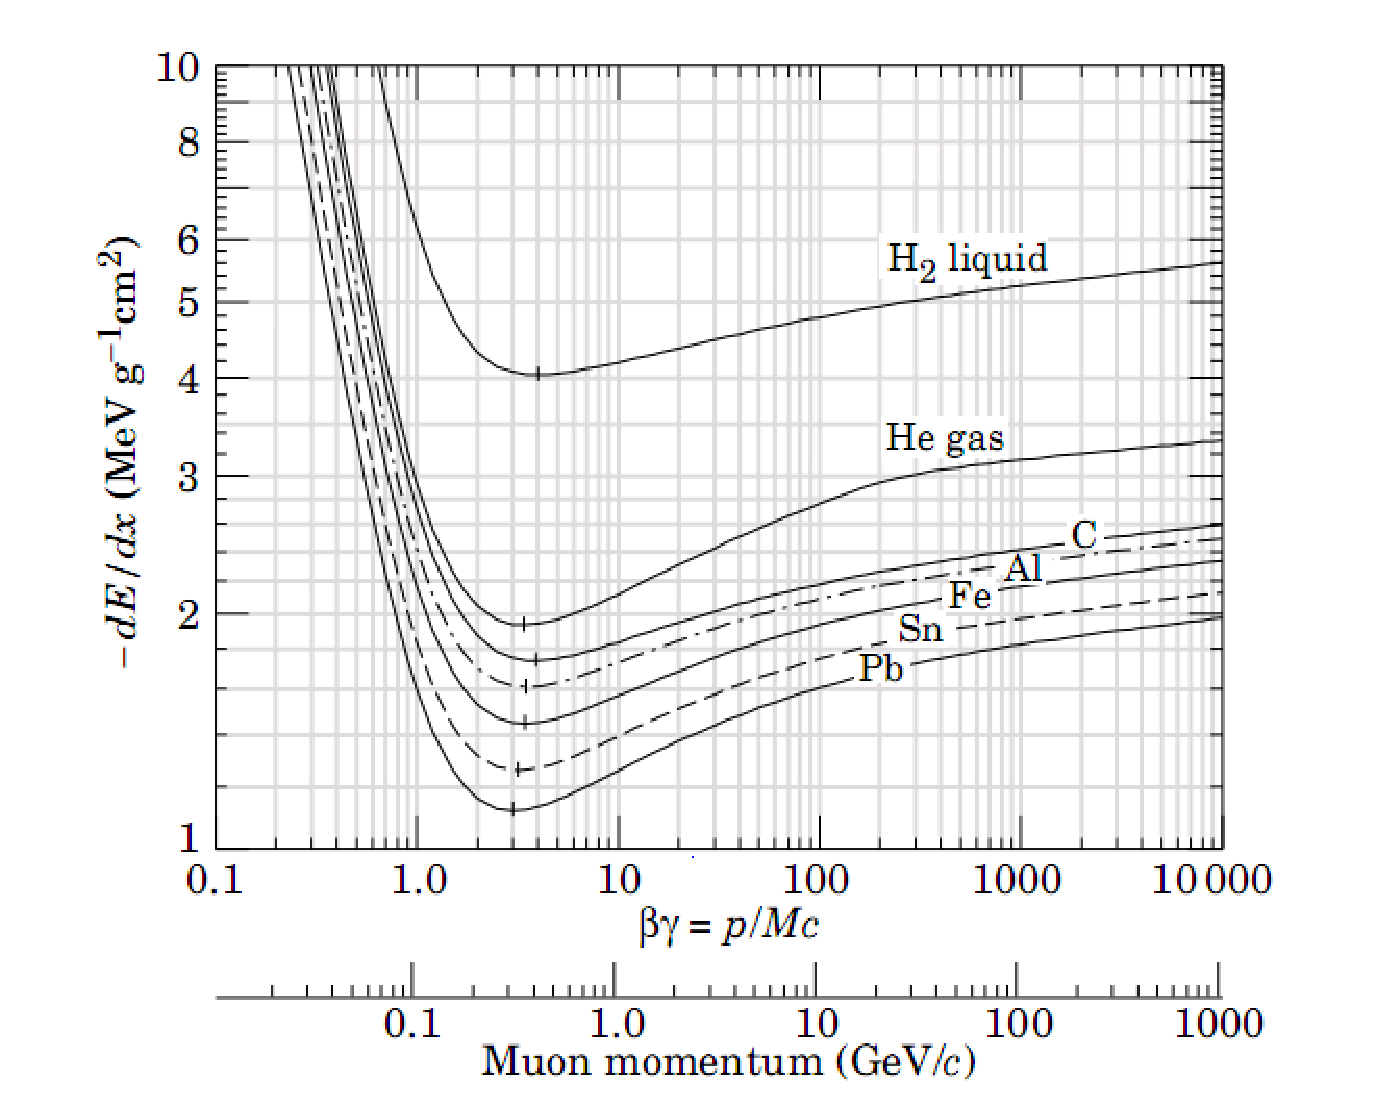
\includegraphics[width = 130mm]{figures/energy_loss.eps}
\caption{\small{Mean energy loss in various materials \cite{yao.}}}
\label{figure:dEdx}
\end{center}
\end{figure}

\subsection{Mass Error Analysis}

The density of the scintillator material was found to be $1.08 \pm
0.09$ g/cm$^3$. The height was $2.5 \pm 0.2$ cm, the large errors due
to the tape around the scintillator making it difficult to measure the
dimensions and density.

The mode of the distribution of muons passing through was $9.8 \pm 0.5
\times 10^{-2}$ V.  Combined with the value of $E_min$ from
\ref{minionizationenergy}, this gives the converstion ratio to be

\begin{equation} VtoMeV = 51 \pm 7 \mathrm{ MeV/V} \end{equation}   

where the errors are independent and thus added in quadrature.

The maximum detected electron pulse peak voltage was determined to be
$V_{max}^e = 1.2 \pm .1$ V, resulting in a maximum electron kinetic
energy of $61\pm 10.$ MeV. Thus, the mass of the muon was established
to be $122 \pm 20.$ MeV. 
